\chapter{Producing a Schedule} \label{cha:analysis}
In this chapter we will describe the process of making a system capable of constructing a schedule for nanosatellites. We will define and describe an input-language, construct a model capable of creating said model, and explain relevant theory for creating such system.

We have chosen to use the GomX-3 nanosatellite as context for this project. The context will help us to make decisions in regards to how we solve the problems we will be facing, and help us make examples throughout the report. The nanosatellite have been described in \textbf{Bisgaard et al. 2016}\cite{gomx3} and we have modelled our payloads and other aspects based on this.

\section{Solution} \label{sec:solution}
The solution we propose to the problem statement, introduced in the introduction, is a follows:
\begin{itemize}
	\item	Input a payload description file that specifies all of the payloads, and input some parameters that specifies the environment and validation options
	\item	Produce a \gls{cora} model that will find the a near optimal schedule in regards to profit while guaranteeing the battery level will never fall below a curtain level
	\item	Validate the schedule in \gls{smc} to test the robustness and act accordingly to the result as well as getting a more accurate simulation of the battery consumption
	\begin{itemize}
		\item	Rejected: modify the input and produce a new schedule for validation
		\item	Accepted: output schedule along with relevant values
	\end{itemize}
\end{itemize}

By doing so we are able to produce a schedule that schedules the payloads and is verified in regards to the robustness.
How the schedule is generated and how the robustness is tested will be explained in the following chapters of this report.
Prior to defining the input language in \cref{sec:read_input} \nameref{sec:read_input}, we will present our tool-chain which provides an overview of how the final system will work and how the different tools are used.

\subsection{Tool-chain} \label{subsec:tool_chainv}
In order to clarify our usage of different tools we will describe the different steps in our system. 
\Cref{fig:tool1} displays a flowchart representation of the tool-chain.

\begin{figure}[h]
	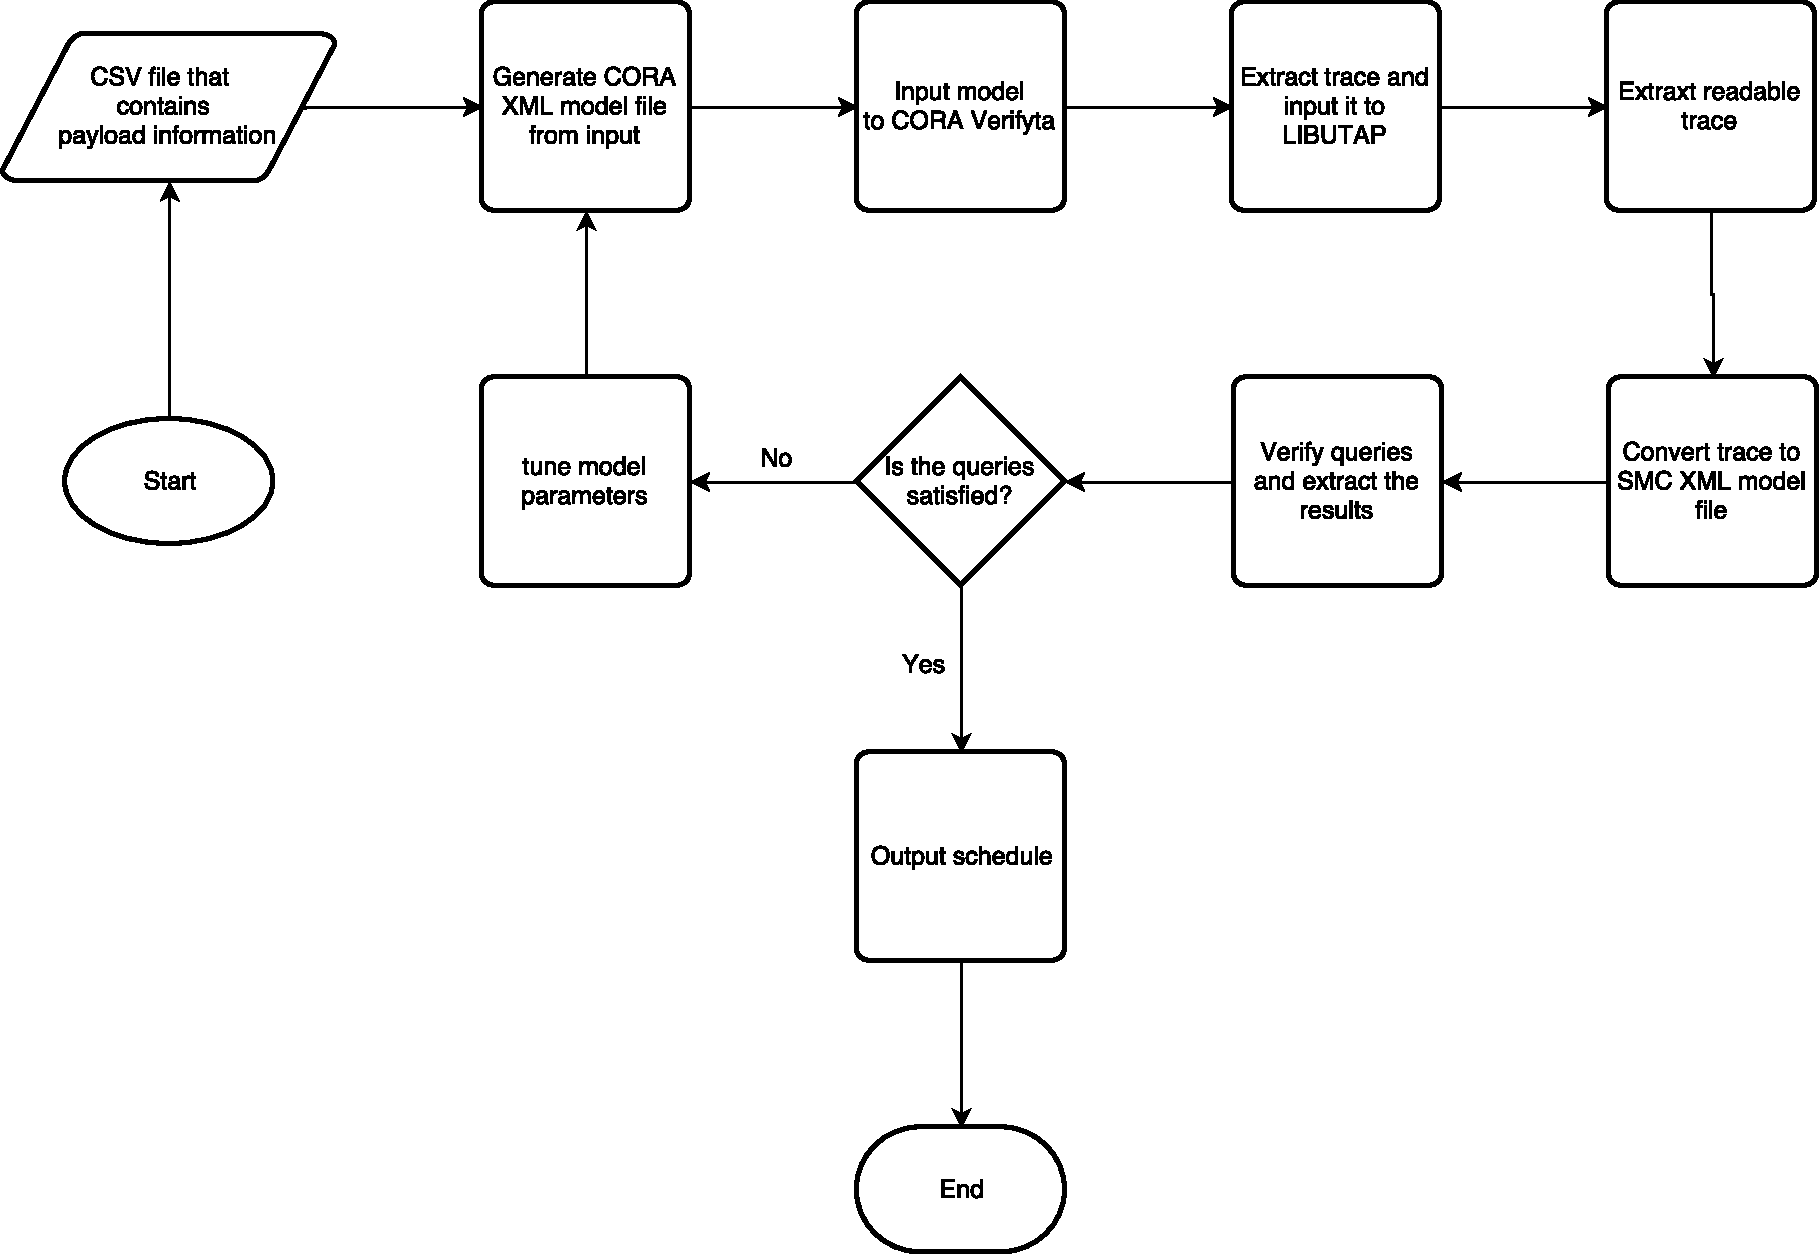
\includegraphics[width=\textwidth]{graphics/tool_chain.pdf}
	\label{fig:tool1}
	\caption{Flowchart that displays the workflow and use of tools}
\end{figure}

\paragraph{Location 1 - CSV file that contains payload information} 
Is the input file for the system. 
The usage of this file and its format is described in \cref{sec:read_input}.

\paragraph{Location 2 - Generate \gls{cora} XML models file from input} 
In this location we will read the CSV file or the tuned parameters from location 9. 
The input is used to generate two \gls{cora} models.
The values specified in the input file can be in a range to indicate variations or uncertainties in how much time, power, etc. a payload uses.
One model uses the worst case values and the other will use the interval. 

%\paragraph{Location 3 - Input model to CORA Verifyta} the Verfyta will generate a trace for each model.

\paragraph{Location 4 - Test worst case model} 
Run the queries on the worst case model.

\paragraph{Location 5 - Is the worst case possible?} 
If we were unable to produce a trace for the worst case, we will not be able to guarantee that any of the schedules we produce will stay within the specified parameters. 
We will as a result thereof go to location 6, the fail state.

\paragraph{Location 7 - Extract trace from the \gls{cora} model and it to \acrshort{lbtp}} 
In this location we will extract a trace from the \gls{cora} model and use it as input for the tracer function in \acrshort{lbtp}. 
The tracer function will transform the output into a readable trace which can be used later on.

%\paragraph{Location 9 - Convert trace to \gls{smc} xm model file} in this location we will read the trace and produce the \gls{smc} model that will be used in the next location.

\paragraph{Location 10 - Verify queries and extract the results} 
The \gls{smc} Verifyta will run the queries on the \gls{smc} model and output the results, see \cref{sec:smc}. 
These queries is made to validate and test the robustness of the trace.

\paragraph{Location 13 - Output schedule} 
If the queries are satisfied we will output the schedule, as this will indicate that the trace, or schedule, is correct.

\paragraph{Location 12 - Tune model parameters} 
If the queries were not satisfied, the schedule will be discarded and we will produce a new one. 
In order to produce a new schedule, we will provide \gls{cora} with a new set of parameters based on those from the CSV file. 
These parameters will be loyal to those specified in the CSV file, but their ranges will be shortened in order to provoke new choices in the schedule. 
This will change the workflow as we are not interested in verifying the worst case model any more, as the previous worst case is still true to this version of the parameters. 
We will therefore skip location 4, 5, and 6 and will go directly yo location 7.


\section{Schedule} \label{sec:schedule}
In order to produce a schedule we will first have to define what is considered a viable schedule. Different considerations goes into this, most impotently what is the requirements for a reliable schedule? The produced schedule should be correct and validated according to the specifications given as input.

First we will discuss what type of real-time the satellite is considered to be. It may be considered soft real-time, which means that if some deadlines fails it is not mission critical, it should however not be a common occurrence. In favour of the system being hard real-time is that the satellite can only perform some payloads within certain windows of time, such as communicating with earth, and must at that point be available to receive new schedules. \textit{As there are both soft- and hard real-time aspects to the satellite mission, it will be considered weakly hard real-time. This means that some deadlines must be upheld, where as others are not of the same level of importance.}

The schedule will need to be robust, meaning being capable of handling errors, such as; the satellite will sometimes have to restart at unforeseen times, or maybe the moon blocks the sun and the battery would therefore not recharge as much as expected. This may cause the satellite to fall behind schedule and would in some way need to compensate for this.
The battery level will have to be considered at all times, when producing and validating the schedule, and may never fall below a specified level, as it results in the satellite entering a safe mode where only the most necessary processes are allowed.
Therefore the schedule must accommodate this in a way such that there are no risk of the power level ever falling below the specified level.

A schedule is considered viable if it upholds the following criteria
\begin{enumerate}
	\item Battery level must at all times be above a certain level
	\item Schedule must give instructions from start to end
	\item Schedule must be optimal in regards to profit, while upholding other requirements such as battery level
\end{enumerate}
The first requirement will be referred to as a threshold and must be specified by the user during configuration.\\
The second requirement is there to allow the user to inspect every single step of the schedule, from start to end.\\ 
The goal of the third requirement is make sure that the nanosatellite are doing something worthwhile. This is why we introduce the profit aspect which should reflect actions that provides value, such as collecting data.

% Weakly hard
% http://ieeexplore.ieee.org/stamp/stamp.jsp?arnumber=919277
% Reasoning: We can do a lot of things whenever, but have to send data in surtain windows, and must receive new schedules at some point
\section{Reading the Input} \label{sec:read_input}
In order to model the payloads, battery, and schedule properties, we will need some information from the user.
The payloads are described through an input file where the dimensions represents the variables which will be used when producing the schedule.
The other properties related to the nanosatellite, is described in a configuration file.\\
We have filled out both files to provide examples of how to use them. It is expected that the user sets all of the variables in order to represent their system.

\subsection{Payload Specification} \label{subsec:csv}
The payloads are defined by eight variables and are defined in a CSV file. An example of this file with five payloads can be seen in \cref{lst:csv}. 
These payloads are based on those from the GomX-3 nanosatellite\cite{gomx3}.\\
The eight variables are Name, Time, Energy, Profit, Deadline, Dependencies, Window, and MaxRuns.\\
\textbf{Name} should indicate what the payload represents. When modelled, a payloads name will be translated into a number in range 0 to N-1 where N is the amount of payloads. The numeric name will also be used when a payload is referenced in the produced schedule.\\
\textbf{Time} specifies how much time, in minutes, it will take to complete the payload. It is defined by a range in order to allow for uncertainty in regards to the timing of the payloads. It is valid to specify a number that is higher than the orbit duration, but a time may not be below 0.\\
\textbf{Energy} specifies how high a load, in mAh, the payload applies on the battery every minute it is being executed.\\
\textbf{Profit} is expressed within a range from 1 to 5, which signifies how valuable or profitable it is to complete a payload. 1 being the least profitable and 5 being the most. In the example from below, L1 and L2 represents the use of the L-Band transmitter that the GomX-3 nanosatellite use to communicate with other satellites, which allows it to collect valuable data. Which is why it has been given a profit of 5 as it is the most profitable payload. The first payload Slew represents the action of slewing the nanosatellite. This does not directly generate any profit for the nanosatellite as no data is gathered.\\
\textbf{Deadline} is a positive integer and is used to cancel payloads which are delayed too much. The minimum value for the deadline is that of the maximum execution time and the maximum is undefined. The scheduler may chose to wait before executing a payload and we can therefore risk that it is no longer relevant to execute the next payload in the queue.
The decision for whether or not to cancel a payload in regards to its deadline goes as follows: \textit{if the time we have spent waiting for the next payload to start plus the time it takes to complete the payload exceeds the deadline; then cancel}. We want to make sure that only payloads that are guaranteed to finish within their deadline start\\
\textbf{Dependencies} contains a list of other payloads which the current payload is waiting for to be completed. A payload may only be executed if all payloads expressed in its dependencies have previously been activated. The user may specify a dependency of multiple executions of another tasks. In the example, X is dependant on L1 and L2 to be completed twice, before it may self be executed.\\
Some payloads can only be executed in a certain time \textbf{Window}, such as when they are above the communication station on Earth.
This is why we have added the variable which restricts when payloads can be executed as it may only happen within the window. The window is specified by a range with the minimum value of 0 and the maximum is equal to the the orbit time. If a payload does not have an associated window it will be allowed to run at any given time, given its dependencies are fulfilled.\\
In addition we have added the concept of \textbf{MaxRuns} which indicates the amount of times each payload can be executed in a payload cycle. A payload cycle is completed when all of the payloads have been executed as many times as described by their MaxRuns value. Whenever a payload has been completed an associated counter, that belongs to the payload, is incremented. When all payloads have reached the MaxRuns value, their individual counter is set to $0$ and a new payload cycle begins. All dependencies are also being reset when a new cycle begins, which means that payloads will need to wait for their dependencies to be completed again. This is done to avoid executing the same payload for the duration of the schedule as soon as its dependencies are fulfilled. MaxRuns is a constant and all payloads must be set to $1$ or higher.
\begin{figure}[H]
\begin{lstlisting}[caption={Example of how five payloads can be defined}, label=lst:csv, language=text]
Name,	Time,	Energy,	Profit,	Deadline,	Dependencies,Window,MaxRuns
Slew,	2-5,	10,		1,		85,			-1,			-1,		3
L1,		90-90,	20,		5,		120,		-1,			-1,		3
L2,		90-90,	20,		5,		120,		-1,			-1,		2
X,		15-15,	10,		3,		30,			0 2 2 0 0,	45-60,	2
UHF,	15-15,	15,		1,		45,			0 0 0 1 0,	20-65,	1
\end{lstlisting}
\end{figure}

\subsection{Configuration Specification} \label{subsec:init}
The nanosatellite and its battery is specified by a configuration which consists of a list of variables and constants. The configuration is read from an INI file which we have provided an example of below in \cref{lst:ini}.
The configuration is divided into three sections System, CORA, and SMC.\\
The System specific variables describes the nanosatellite and the time constraints.
The variables are:
\begin{itemize}
	\item schedule\_length
	\item orbit\_time
	\item battery\_capacity
	\item idle\_cost
	\item safe\_threshold
	\item soc
	\item rec\_rate
\end{itemize}
The \textbf{schedule\_length} defines how long the produced schedule should be, in minutes. 
\textbf{orbit\_time} defines how long it takes to complete one orbit, in minutes. 
The \textbf{battery\_capacity} is an constant that defines the maximum capacity of the battery. We do not expect that the user defines every single operation that the nanosatellite is capable of performing, which is why we have made an abstraction by introducing the \textbf{idle\_cost} variable. 
\textbf{idle\_cost} is the load that is imposes on the battery at all times, even when the nanosatellite is idling, not currently executing any of the defined payloads.
This will allow us to disregard some of the payloads that the nanosatellite may perform as they can be grouped together as one single background process which is always being executed.
The user should only consider payloads which can be executed in parallel to the defined payloads and only chose those which energy and time cost are trivial.
Failing to do so may result in a non representative model of their nanosatellite and therefore a schedule where our guarantees may not be valid.\\
Based on the findings from Bisgaard et al. 2016\cite{gomx3} we have decided to include the \textbf{safe\_threshold} variable.
This variable is used to determine when the nanosatellite's \gls{soc} is too low to continue executing the schedule.
If the nanosatellite go below this threshold, it is in danger of depleting the battery, which means it will not be able to communicate with Earth for a period of time.
This will result in a huge loss of potential profit as we are no longer able to execute profitable payloads and should therefore be avoided.It is critical that the schedules we produce will never go below this threshold.\\
\textbf{rec\_rate}  defines the recharge rate such that the value is added to the battery's capacity every minute that the nanosatellite is in insolation.\\
We have three variables that are related to the \gls{smc} model where two of them is used in its battery model.\\
\begin{itemize}
	\item f\_rate
	\item ac\_width
	\item certainty
\end{itemize}
\textbf{f\_rate} is a rate that is specific to the battery model we have chosen, and it is used to simulate the recovery effect of batteries. The recovery effect will be described later in \myref{sec:kibam}, together with the \textbf{ac\_width} constant.
The constant \textbf{certainty} specifies how certain we require that \gls{smc} should be in its results. \gls{smc} is described in \myref{sec:smc}.
\begin{figure}[H]
\begin{lstlisting}[caption={Example of how the environment can be defined}, label=lst:ini, language=text]
[SYSTEM]
# System specific
# schedule length in minutes
schedule_length = 720
# orbit time in minutes
orbit_time = 90
# battery capacity in mAh
battery_capacity = 5400
# idle cost in mAh
idle_cost = 1
# safe mode threshold in percentage [0-100]
safe_threshold = 40
# The start SoC in mAh
soc = 4800

[CORA]
# Cora specific

[SMC]
# SMC specific
# Recharge rate
rec_rate = 4.2
# flow of available charge
f_rate = 0.0002324
# available width in relation to bound width
ac_width = 0.16667
# how certain should the system be in the results? Percentage [1-99]
certainty = 95
\end{lstlisting}
\end{figure}
At this point the CORA section does not contain any variables, the section is used as a placeholder for future versions of the system, as the model could be expanded to include variables specific to \gls{cora}.

Now that payloads and nanosatellite is specified, we are able to start modelling the system.

\section{UPPAAL} \label{sec:uppaal}
We have chosen to use \acrlong{cora}\cite{cs_cora}\cite{cora_tutorial} and \acrlong{smc}\cite{smc_home}\cite{cs_smc} for producing and verifying the schedule. We will describe the common charismatics for both versions and then introduce them before their respective models are presented.

Common for all versions of UPPAAL, is that; it has global decelerations and templates. 
An example template can be seen in \cref{fig:uppaal_eksample}.
One model may have several templates, each with its own local decelerations. The template itself consists of one to many locations and edges that connects the locations.\\
One location in each template must be initial in order for UPPAAL to determine the starting state. In addition a location can be urgent, meaning time is not allowed to pass while the location is active, or committed which is a stronger expression than urgent. Committed indicates that activating an outgoing transition is of priority. If any committed location in the model is part of the current state, at least one transition from a committed location must be part of the next transition.
Edges may be decorated with; selects, guards, synchronizations, and updates. 
Selects are used for introducing new temporary variables, and are coloured yellow.
Guards are used to ensure that an edge is not activated prematurely, and are coloured green.
Synchronizations are used for activating multiple edges across templates simultaneously, and are coloured light blue. If an exclamation mark is used, it indicates that it is calling a synchronisation, whereas a question mark is receiving one.
Finally updates are used to change variable values, and to call functions written in declarations, and are coloured dark blue.\\
Locations can be given a name and an invariant. An invariant must always be evaluated to true e.g. if a location have the invariant $time <= 5$, at time five there will be a chance of state. Invariants are coloured pink.\\
Also common for the versions of UPPAAL, is that queries can be written in order to ensure sustain properties are upheld, such as; is some location reachable, and will time ever exceed some amount.

\begin{figure}[h]
   \centering
   \begin{tikzpicture}
   %Locations
   \node [init, label = {
           [align=left]above:
           \textcolor{name}{location A}
       }] (l0) {$\cup$};
   \node [location] (l1) [right of=l0, xshift=30mm, label={
        [align=right]above:
       \textcolor{name}{Location B}\\
       \textcolor{invariant}{x <= myLimit}}
   ] {};
   \node [location] (l2) [right of=l1, xshift=40mm, label={
       [align=right]above:
       \textcolor{name}{location C}
   }] {};

   \path[->,black, thick] (l0) edge node [midway, below ][align=center]{\textcolor{update}{mayRun()}} (l1);
   \path[->,black, thick] (l1) edge node [midway, below][align=center]{
   \textcolor{select}{a: int[0,N-1]}\\
           \textcolor{guard}{everythingIsGood() == true}\\
           \textcolor{sync}{ready!}\\
           \textcolor{update}{changeValue(), myVar = a}} (l2);
   \end{tikzpicture}
   \caption{Example template}
   \label{fig:uppaal_eksample}
\end{figure}

\section{UPPAAL CORA}\label{sec:upp_cora}
UPPAAL \acrfull{cora} is a branch of UPPAAL, that uses linearly priced timed automata to find optimal paths satisfying certain goals, based on lowest accumulated cost\cite{cs_cora}. Cost is a variable that can be only be interacted with through locations, where it is possible to define the incremental rate with which it will grow, with the passing of time. 
Which means that if a location's rate is 5, and two time units passes, the cost will grow by 10. It allows \gls{cora} to prune traces, if two traces reach the same location where all variables for each of the traces are identical expect for the cost variable, the trace with the lowest cost will be kept to preserve memory. 
Due to the underlying structure of \gls{cora} it is only possible to do reachability checks, and does not allow for liveness or deadlocks checks.
Only best first search is supported when we are searching for the best trace. Lastly \gls{cora} cannot guarantee termination unless the modelled system is acyclic and clocks are bound by invariants.

\Gls{cora} have been used in a range of problems regarding scheduling problems, the most related case for our problem is GomX-3 case, where they used \gls{cora} to generate a battery aware schedule for CubeSat satellite. Their solution takes a set of parameters to generate fractions of the entire schedules and, when all parts of the schedule is generated, they are assembled by appending them in a chronological order. Lastly, the acummulated schedule is tested with an external \gls{kibam} battery model.

\Gls{cora} introduced the concept of cost, which as mentioned is accumulated over time. An example of how such a model may look can be seed in \cref{fig:cora_eks}.

\begin{figure}[H]
	\centering
	\begin{tikzpicture}
	%Locations
	\node [init] (l0) [label={
		[align=left]above:
		\textcolor{name}{A}
	}, label={
		[align=left]left:
		\textcolor{invariant}{cost '== 1}\\
		\textcolor{invariant}{\&\& time <= 5}
	}] {};
	\node [location] (l1) [right of=l0, xshift=20mm, yshift=20mm, label={
		[align=left]above:
		\textcolor{name}{B1}
	}, label={
		[align=left]below:
		\textcolor{invariant}{cost '== 1}\\
		\textcolor{invariant}{\&\& time <= 5}
	}] {};
	\node [location] (l2) [right of=l0, xshift=20mm, yshift=-20mm, label={
		[align=left]above:
		\textcolor{name}{B2}
	}, label={
		[align=left]below:
		\textcolor{invariant}{cost '== 1}\\
		\textcolor{invariant}{\&\& time <= 5}
	}] {};
	\node [location] (l3) [right of=l2, xshift=20mm, yshift=20mm, label={
		[align=left]above:
		\textcolor{name}{C}
	}, label={
		[align=left]right:
		\textcolor{invariant}{cost '== 1}\\
		\textcolor{invariant}{\&\& time <= 5}
	}] {};
	%Edges
	\path[->,black, thick] (l0) edge node [midway, left][align=left]{
			\textcolor{guard}{time >= 3}} (l1);
	\path[->,black, thick] (l0) edge node [midway, left][align=left]{
			\textcolor{guard}{time >= 3}} (l2);
	\path[->,black, thick] (l1) edge node [midway, right][align=left]{
			\textcolor{guard}{time >= 10}} (l3);
	\path[->,black, thick] (l2) edge node [midway, right][align=left]{
			\textcolor{guard}{time >= 7}} (l3);
	\end{tikzpicture}
	\caption{Simple model made in \gls{cora}, which displays an increase in cost over time}
	\label{fig:cora_eks}
\end{figure}

In \cref{fig:cora_eks} we see a \gls{cora} model with four locations and four edges connecting them. On three of the location there is an invariant bound to the clock "\uppVar{time}" and an associated cost rate. While in the initial location "\uppLoc{A}" the cost rate is one meaning that for every unit of time spend in this \uppLoc{A} the cost will increase by one, it will stay in \uppLoc{A} for three to five units of time before moving on to the next location.\\
After this is where the model gets interesting, there are at this point two possible transitions, it may move to either "\uppLoc{B1}" or "\uppLoc{B2}". In \uppLoc{B1} the cost will increase with a rate of 3 per unit of time and will stay there until time reaches ten. Alternatively it may transition to \uppLoc{B2} where the cost rate is four and will stay there until time is between seven and ten. After visiting one of these locations it will reach the final state "\uppLoc{C}". \\
In UPPAAL we can then run the query seen in \cref{eq:cora_get_c}, a simple query asking if location \uppLoc{C} is reachable, however in \gls{cora} the settings for diagnostic trace allows us to get the best trace, meaning the one with the smallest cost.
\begin{align}
E<> Template.C
\label{eq:cora_get_c}
\end{align}
This is beneficial as the optimal route may not always be what seems to be the obvious one. We see in \cref{fig:cora_eks} that \uppLoc{B1} only have a cost of three per tic whereas \uppLoc{B2} have a cost of four per tic, however it is required to stay in \uppLoc{B1} for a longer period of time, actually causing the bottom route to become cheaper.
The model in \cref{fig:cora_eks} is of course a simple one,

%This can be advantageous for modelling systems such as satellites where energy is an important and limited resource which can be represented by the cost. After running a query it is possible to extract a trace, which can be used to represent the generated schedule.

%http://people.cs.aau.dk/~adavid/cora/download.html#download


%optimal sceduling and planning.
%state-space exploration -> promising and cheap visited first -> prune parts of search tree not improving solution.
%symbolic data structure -> symbolic state-space representation with cost information -> optimal or near-optimal solutions

%S2,3: problem of cost-optimal reachability -> symbolic branch-and-bound solving this problem.
% clocks are non-negative real values, can be reset and grow at a fixed rate.

%S5: PTA-related optimization problems -> future support


\section{Battery Models} \label{sec:kibam}
Part of the proposed solution is to ensure that battery level are maintain at an expectable level, in order to do this we need some way of modelling a battery, this section will go over three different battery models to determine what drawbacks there may be when using certain battery models. An important factor to consider when examining the battery models is the recovery effect, which can have large impact on the expected lifetime\cite{battery_model}. Recovery effect happen after a battery has been discharged for a period of time, the amount of current applied to the battery effects the recovery effect along with the battery capacity. The performance of the different models will be compared to the actual measured of a lithium-ion battery, measured are taken from \cite{battery_lifetime_analysis}, unfortunatly we are unable to obtain the specification for the lithium battery used in the paper as they are not listed in the paper. The measures for the different battery models is taken from \cite{battery_model} which also uses the same battery specification as the other paper they claim.

The Ideal model is very simplistic due to it only having two variables to determine the batteries lifetime(L), capacity(C) and load current(I). Capacity relates to the batteries amount of amp-hours, and load current is the constant discharge on the battery in amps. The formal for this is shown in \cref{eq:bm}.

\begin{equation}\label{eq:bm}
L=C/I
\end{equation}

Performance of the Ideal model can be seen in \cref{table:t-Ideal}. The table is divided into two parts, constant load and variable load, the column ``Meas, min'' show the actual measured readings of the lithium-ion battery under different loads. To the right the Ideal estimation are shown. In general the Ideal model overestimate the expected lifetime in all cases, shown in T1 the deviation from the actual measures differs by 28.58\%, a trend seems to appear in that lower amps often results in better predictions from the Ideal model with constant loads. Only T5 and T6 dose not apply to this, because T5 have a better prediction then T6 even though T5 has a higher load. During variable loads all cases overestimate by a substantial amount, the closest approximation is C5 during variable loads with a 18.5\% overestimation. The data shows that the Ideal model does a poor job of estimating the actual lifetime of a battery, which is properly because the Ideal model assumes linear effect for lifetime estimation. Additionally for variables loads the Ideal model does not consider recovery effect of the battery which further deviate results from the measured values. 

% Please add the following required packages to your document preamble:
% \usepackage[table,xcdraw]{xcolor}
% If you use beamer only pass "xcolor=table" option, i.e. \documentclass[xcolor=table]{beamer}
\begin{table}[H]
	\centering
	\scalebox{0.8}{
	\begin{tabular}{|llllll|lllll|}
		\hline
		\multicolumn{6}{|c|}{Constant load} & \multicolumn{5}{c|}{Variable load} \\ \hline
		\rowcolor[HTML]{EFEFEF} 
		\multicolumn{1}{|l|}{\cellcolor[HTML]{EFEFEF}Test} & \multicolumn{1}{l|}{\cellcolor[HTML]{EFEFEF}I, amps} & \multicolumn{1}{l|}{\cellcolor[HTML]{EFEFEF}Meas, min} & \multicolumn{1}{l|}{\cellcolor[HTML]{EFEFEF}Ideal, min} & \multicolumn{1}{l|}{\cellcolor[HTML]{EFEFEF}$\Delta$T} & \%$\Delta$ & \multicolumn{1}{l|}{\cellcolor[HTML]{EFEFEF}Test} & \multicolumn{1}{l|}{\cellcolor[HTML]{EFEFEF}Meas, min} & \multicolumn{1}{l|}{\cellcolor[HTML]{EFEFEF}Ideal, min} & \multicolumn{1}{l|}{\cellcolor[HTML]{EFEFEF}$\Delta$C} & \%$\Delta$ \\ \hline
		T1 & 222.7 & 141.0 & 181.3 & 40.3 & 28.58\% & C1 & 54.5 & 70.8 & 16.3 & 29.91\% \\ \hline
		\rowcolor[HTML]{EFEFEF} 
		T2 & 204.5 & 156.6 & 197.4 & 40.8 & 26.05\% & C2 & 73.3 & 91.9 & 18.6 & 25.38\% \\ \hline
		T3 & 108.3 & 307.8 & 372.8 & 65 & 21.12\% & C3 & 88.3 & 108.5 & 20.2 & 22.88\% \\ \hline
		\rowcolor[HTML]{EFEFEF} 
		T4 & 107.5 & 312.0 & 375.6 & 63.6 & 20.38\% & C4 & 136.0 & 163.0 & 27 & 19.85\% \\ \hline
		T5 & 94.9 & 358.2 & 425.4 & 67.2 & 18.76\% & C5 & 182.7 & 216.5 & 33.8 & 18.50\% \\ \hline
		\rowcolor[HTML]{EFEFEF} 
		T6 & 84.3 & 397.2 & 478.9 & 81.7 & 20.57\% & C6 & 59.0 & 74.7 & 15.7 & 26.61\% \\ \hline
		T7 & 75.5 & 448.2 & 534.8 & 86.6 & 19.32\% & C7 & 51.1 & 66.9 & 15.8 & 30.92\% \\ \hline
		\rowcolor[HTML]{EFEFEF} 
		T8 & 28.0 & 1248 & 1442 & 194 & 15.54\% & C8 & 55.0 & 70.8 & 15.8 & 28.73\% \\ \hline
		T9 & 19.5 & 1818 & 2071 & 253 & 13.92\% & C9 & 54.9 & 70.8 & 15.9 & 28.96\% \\ \hline
		\rowcolor[HTML]{EFEFEF} 
		T10 & 3.0 & 12690 & 13458 & 768 & 6.05\% & C10 & 142.7 & 171.3 & 28.6 & 20.04\% \\ \hline
	\end{tabular}}
	\caption{Comparison of actual measure and measures from Ideal model. Specification for the variable loads can be found in \cref{table:variable_loads_list}
	}
	\label{table:t-Ideal}
\end{table}

Peukert Model introduces a few new variables in comparison to the Ideal model, like the previous we still want to estimate the expected lifetime, but to better represent the battery a non-linear model is needed. Peukert fixes this by changing the formula to what is seen in \cref{eq:pm}. 

\begin{equation}\label{eq:pm}
L=(\frac{C}{I^k})
\end{equation}
\begin{itemize}
	\item L - lifetime in hours
	\item C - capacity in AH
	\item I - load current in amps
	\item k - Peukert Exponent
\end{itemize}

Unlike the previous model these parameter not as concrete. Acording to \cite{battery_modeling} C should be close to the value of the battery capacity and k should be between 1.2 and 1.7 to give the best results. This should be noted that this is only for constant loads. as it best illustrate how Peukert model functions\cite{battery_modeling}. k can sometimes be provided by the manufactors, since it can be hard to determine the exact value of k without actual testing a battery

\cref{table:t-Peukert} showcases the estimations using Peukert. In most cases Peukert overestimate except for one instance in test T10, it underestimate with 3.17\%. It seems to become more accurate the smaller the amps are, with the outlines, T5 and T6 Similarly to \cref{table:t-Ideal}. One thing to notices is that for variable loads it still has a high mismatch compared to measured values, this is due to Peukerts model not taken recovery effect into account. But overall Peukert performance better than the Ideal model.

\begin{table}[H]
	\centering
	\scalebox{0.8}{
	\begin{tabular}{|llllll|lllll|}
\hline
\multicolumn{6}{|c|}{Constant load} & \multicolumn{5}{c|}{Variable load} \\ \hline
\rowcolor[HTML]{EFEFEF} 
\multicolumn{1}{|l|}{\cellcolor[HTML]{EFEFEF}Test} & \multicolumn{1}{l|}{\cellcolor[HTML]{EFEFEF}I, amps} & \multicolumn{1}{l|}{\cellcolor[HTML]{EFEFEF}Meas, min} & \multicolumn{1}{l|}{\cellcolor[HTML]{EFEFEF}Peukert, min} & \multicolumn{1}{l|}{\cellcolor[HTML]{EFEFEF}$\Delta$T} & \%$\Delta$ & \multicolumn{1}{l|}{\cellcolor[HTML]{EFEFEF}Test} & \multicolumn{1}{l|}{\cellcolor[HTML]{EFEFEF}Meas, min} & \multicolumn{1}{l|}{\cellcolor[HTML]{EFEFEF}Peukert, min} & \multicolumn{1}{l|}{\cellcolor[HTML]{EFEFEF}$\Delta$C} & \%$\Delta$ \\ \hline
T1 & 222.7 & 141.0 & 154.5 & 13.5 & 9.57\% & C1 & 54.5 & 60.5 & 6 & 11.01\% \\ \hline
\rowcolor[HTML]{EFEFEF} 
T2 & 204.5 & 156.6 & 168.4 & 11.8 & 7.54\% & C2 & 73.3 & 79.1 & 5.8 & 7.91\% \\ \hline
T3 & 108.3 & 307.8 & 321.3 & 13.5 & 4.39\% & C3 & 88.3 & 93.8 & 5.5 & 6.23\% \\ \hline
\rowcolor[HTML]{EFEFEF} 
T4 & 107.5 & 312.0 & 323.7 & 11.7 & 3.75\% & C4 & 136.0 & 142.5 & 6.5 & 4.78\% \\ \hline
T5 & 94.9 & 358.2 & 367.5 & 9.3 & 2.60\% & C5 & 182.7 & 190.2 & 7.5 & 4.11\% \\ \hline
\rowcolor[HTML]{EFEFEF} 
T6 & 84.3 & 397.2 & 414.4 & 17.2 & 4.33\% & C6 & 59.0 & 64.4 & 5.4 & 9.15\% \\ \hline
T7 & 75.5 & 448.2 & 463.6 & 15.4 & 3.44\% & C7 & 51.1 & 56.5 & 5.4 & 10.57\% \\ \hline
\rowcolor[HTML]{EFEFEF} 
T8 & 28.0 & 1248 & 1270 & 22 & 1.76\% & C8 & 55.0 & 60.5 & 5.5 & 10.00\% \\ \hline
T9 & 19.5 & 1818 & 1835 & 17 & 0.94\% & C9 & 54.9 & 60.5 & 5.6 & 10.20\% \\ \hline
\rowcolor[HTML]{EFEFEF} 
T10 & 3.0 & 12690 & 12288 & -402 & -3.17\% & C10 & 142.7 & 148.8 & 6.1 & 4.27\% \\ \hline
\end{tabular}}
	\caption{Comparison of actual measure and measures from Peukert model. Specification for the variable loads can be found in \cref{variable_loads_list}
	}
	\label{table:t-Peukert}
\end{table}

\gls{kibam} uses two wells as an abstract concept to represent a battery. It consist of an available charge and a bound charge as shown in \cref{fig:kibam_wells}, c determines the ratio of the two wells based on the total capacity. Current can only be drawn from the available charge, when the available charges height $h_2$ is lower then bound charge height $h_1$, charge start to flow from bound charge to available charge until both wells are at equal height. The rate of this flow is determined by the value k, this simulate the recovery effect of the battery like previous models was not able to capture. To calculate $y{1}$ and $y{2}$ can be seen in \cref{eq:y1} and\cref{eq:y2} along with a short description of the variables used in these equations.

\begin{figure}[H]
	\center
	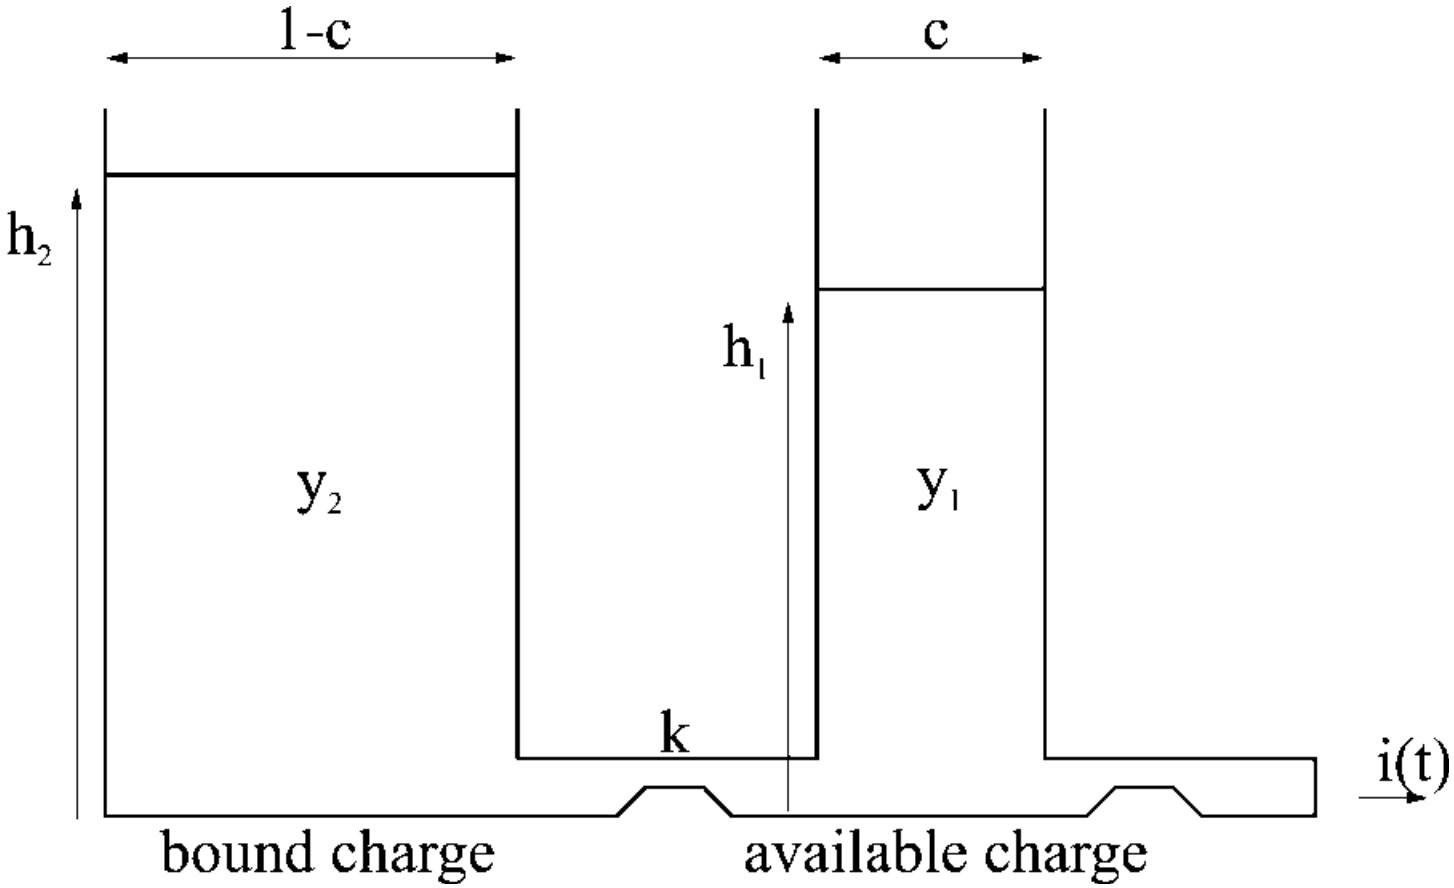
\includegraphics[width=\textwidth/2]{graphics/kibam.jpg}
	\caption{Displays the two wells of \gls{kibam}}
	\label{fig:kibam_wells}
\end{figure}

\begin{equation}\label{eq:y1}
y_1(t) = cCe^{-k't}+\frac{(y_0k'c-I)(1-e^{-k't})}{k'}-\frac{Ic(k't-1+e^{-k't})}{k'}
\end{equation}

\begin{equation}\label{eq:y2}
y_2(t) = (1-c)Ce^{-k't}+y_0(1-c)(1-e^{-k't})-\frac{I(1-c)(k't-1+e^{-k't})}{k'}
\end{equation}

C is capacity in Ah, e is Euler's number, k' is $k/c(1-c)$, k is a constant, t is time in hours, c is the ratio between available and bound charge, and I is the load current applied on the battery.

Performance of \gls{kibam} can be seen in \cref{table:t-KiBaM}. Under constant load the results vary, and he only indicating is that an amps above 110 and below 20 seems to give better results. Interesting for variable loads is that all of the predictions from \gls{kibam} underestimate compared to the measured values, some are fairly high though, like in case C7 it underestimate by 40.31\%.

\begin{table}[]
	\centering
	\scalebox{0.8}{
	\begin{tabular}{|l|lllll|llll|l|}
\hline
\multicolumn{6}{|c|}{Constant load} & \multicolumn{5}{c|}{Variable load} \\ \hline
\rowcolor[HTML]{EFEFEF} 
Test & \multicolumn{1}{l|}{\cellcolor[HTML]{EFEFEF}I, amps} & \multicolumn{1}{l|}{\cellcolor[HTML]{EFEFEF}Meas, min} & \multicolumn{1}{l|}{\cellcolor[HTML]{EFEFEF}KiBaM, min} & \multicolumn{1}{l|}{\cellcolor[HTML]{EFEFEF}$\Delta$T} & \%$\Delta$ & \multicolumn{1}{l|}{\cellcolor[HTML]{EFEFEF}Test} & \multicolumn{1}{l|}{\cellcolor[HTML]{EFEFEF}Meas, min} & \multicolumn{1}{l|}{\cellcolor[HTML]{EFEFEF}KiBaM, min} & $\Delta$T & \%$\Delta$ \\ \hline
T1 & 222.7 & 141.0 & 139.9 & -1.1 & -0.78\% & C1 & 54.5 & 36.3 & -18.2 & -33.39\% \\ \hline
\rowcolor[HTML]{EFEFEF} 
T2 & 204.5 & 156.6 & 156 & -0.6 & -0.38\% & C2 & 73.3 & 55.7 & -17.6 & -24.01\% \\ \hline
T3 & 108.3 & 307.8 & 331.4 & 23.6 & 7.67\% & C3 & 88.3 & 71.4 & -16.9 & -19.14\% \\ \hline
\rowcolor[HTML]{EFEFEF} 
T4 & 107.5 & 312.0 & 334.1 & 22.1 & 7.08\% & C4 & 136.0 & 123.6 & -12.4 & -9.12\% \\ \hline
T5 & 94.9 & 358.2 & 384 & 25.8 & 7.20\% & C5 & 182.7 & 175.7 & -7 & -3.83\% \\ \hline
\rowcolor[HTML]{EFEFEF} 
T6 & 84.3 & 397.2 & 437.5 & 40.3 & 10.15\% & C6 & 59.0 & 41.1 & -17.9 & -30.34\% \\ \hline
T7 & 75.5 & 448.2 & 493.3 & 45.1 & 10.06\% & C7 & 51.1 & 30.5 & -20.6 & -40.31\% \\ \hline
\rowcolor[HTML]{EFEFEF} 
T8 & 28.0 & 1248 & 1401 & 153 & 12.26\% & C8 & 55.0 & 38.1 & -16.9 & -30.73\% \\ \hline
T9 & 19.5 & 1818 & 2029 & 211 & 11.61\% & C9 & 54.9 & 34.8 & -20.1 & -36.61\% \\ \hline
\rowcolor[HTML]{EFEFEF} 
T10 & 3.0 & 12690 & 13417 & 727 & 5.73\% & C10 & 142.7 & 131.7 & -11 & -7.71\% \\ \hline
\end{tabular}}
	\caption{Comparison of actual measure and measures from \gls{kibam}. Specification for the variable loads can be found in \cref{variable_loads_list}
	}
	\label{table:t-KiBaM}
\end{table}

Looking at all the results for the three battery models, it show that Peukerts model give overall better estimation for variable loads then Ideal and \gls{kibam}. But the advantage of using \gls{kibam} over Peukerts model under variable load is that \gls{kibam} seems always underestimate, which is good for our case, that ensure that we will never run into a case where the prediction cause the actual system to run out of energy. The Ideal is inferior to Peukerts and \gls{kibam} in almost all predictions, a summarize of the three different battery models can be found below.
\begin{itemize}
	\item Ideal model - linear representation of the battery with no support of recovery effect
	\item Peukert model - non-linear representation of the battery with no support of recovery effect
	\item \gls{kibam} - abstract representation of the battery with support of recovery effect
\end{itemize}
Since CORA can not use \gls{kibam} or Peukert model because \gls{cora} only support price with a linear rate and only natural numbers. The Ideal model will have to suffice.

\section{Cora Model} \label{sec:cora}
The \gls{cora} model takes a set of tasks with some rules and constrains in order to generate a schedule that upholds the specifications. These are fed to the model from the csv file via our own translator.



\subsection*{Task}
\begin{figure}
	\centering
	\begin{tikzpicture}
	%Locations
	\node [init] (l0) {$\cup$};
	\node [location] (l1) [right of=l0, xshift=40mm] {$\cup$};
	\node [location] (l2) [right of=l1, xshift=40mm, label={
		[align=left]right:
		\textcolor{name}{ready}
	}] {$\cup$};
	\node [location] (l3) [below of=l1, yshift=-40mm, label={
		[align=left]left:
		\textcolor{name}{idle}
	}] {};
	\node [location] (l4) [below of=l2, yshift=-40mm, label={
		[align=left]right:
		\textcolor{name}{running}
	}] {};
	\node [location] (l5) [above of=l2, yshift=40mm] {C};
	\node [location] (l6) [above of=l1, yshift=40mm] {};
	\path[->,black] (l0) edge node [midway, below left][align=left]{\textcolor{update}{mayRun()}} (l1);
	\path[->,black] (l1) edge node [midway, above][align=left]{
		\textcolor{select}{a: int[0,N-1]}\\
		\textcolor{guard}{runnableCount() > 0}\\
		\textcolor{guard}{\&\& runnable[a] == 1}\\
		\textcolor{sync}{ready!}\\
		\textcolor{update}{mayRun(), active = a}} (l2);
	\path[->,black] (l2) edge node [midway, right][align=left]{
		\textcolor{guard}{runnable[active] == 1}\\
		\textcolor{sync}{run?}\\
		\textcolor{update}{updateBattery(), }\\
		\textcolor{update}{subIdle(), calcCost()}} (l4);
	\path[->,black] (l4) edge node [midway, below][align=left]{
		\textcolor{guard}{x >= taskTimes[active][0]}\\
		\textcolor{update}{subIdle()}} (l3);
	\path[->,black] (l3) edge node [midway, left][align=left]{
		\textcolor{guard}{x >= taskTimes[active][1]}\\
		\textcolor{update}{reset(), dequeue(),}\\
		\textcolor{update}{x = 0, mayRun()}} (l1);
	\path[->,black] (l1) edge node [midway, left][align=left]{
		\textcolor{guard}{runnableCount() == 0}} (l6);
	\path[->,black] (l6) edge node [midway, above][align=left]{
		\textcolor{sync}{win?}} (l5);
	\path[->,black] (l5) edge node [midway, right][align=left]{
		\textcolor{select}{a: int[0,N-1]}\\
		\textcolor{sync}{ready!}\\
		\textcolor{update}{mayRun(), active = a}} (l2);
	\path[->,black] (l2) edge[bend left=45] node [midway, below][align=left]{
		\textcolor{guard}{runnable[active] == 0}\\
		\textcolor{sync}{run?}} (l1);
	\end{tikzpicture}
	\caption{Task template}
	\label{fig:cora_inso}
\end{figure}
\subsubsection*{Scheduler}
\begin{figure}
	\centering
	\begin{tikzpicture}
	%Locations
	\node [init] (l0) [label={[align=left]left:
		\textcolor{invariant}{checkBattery()}
	}] {};
	\node [location] (l1) [right of=l0, xshift=40mm, label={
		[align=left]right:
		\textcolor{invariant}{checkBattery()}
	}] {$\cup$};
	\path[->,black] (l0) edge[bend left=30] node [midway, above][align=center]{
		\textcolor{sync}{ready?}} (l1);
	\path[->,black] (l1) edge[bend left=30] node [midway, below][align=center]{
		\textcolor{sync}{run!}} (l0);
	\end{tikzpicture}
	\caption{Scheduler template}
	\label{fig:cora_inso}
\end{figure}


\subsection*{Insolation}
The implementation of insolation and battery charge can be seen in \cref{fig:cora_inso} with relevant declarations and functions in \cref{lst:insolation_code}. The model consist of two locations \uppLoc{inSun} and \uppLoc{outSun} to ensure that the nanosatellite can only recharge when it has a clear line of sight to the sun. The recharging is done on the looping edge on \uppLoc{inSun} with the function $increaseBattery()$. To minimize the number of states generate through queries recharging will only happen eight times during an orbit. When half of the $OrbitTime$ have passed, the model is forced to take the transition leading to \uppLoc{outSun}, due to the invariants on \uppLoc{inSun} location and guard on the transition. Afterward the next transition is available when ins clock is greater or equal to OrbitTime, in this transition is also were the clocks ins and $splitTime$ is reset.

On line 10 the declaration for $increaseBattery()$ is define, the purpose of this function is to add energy to the battery and make sure we cannot go over the maximum capacity defined on line 2, the if statement check if the potentially added recharge will make the $batteryCap$ go over its limit ($BatteryMax$) then is just assign $batteryCap$ to $BatteryMax$, else we add the recharge amount to $batteryCap$. lastly we reset the clock splitTime.

\begin{figure}
	\centering
	\begin{tikzpicture}
	%Locations
	\node [init] (l0) [label={
		[align=left]above:
		\textcolor{name}{inSun}
	}, label={
		[align=left]left:
		\textcolor{invariant}{splitTime <= OrbitTime / 8}
	}] {};
	\node [location] (l1) [right of=l0, xshift=40mm, label={
		[align=left]above:
		\textcolor{name}{outSun}
	}, label={
		[align=left]right:
		\textcolor{invariant}{ins <= OrbitTime}
	}] {};
	%Edges
	\path[->,black] (l0) edge[bend left=30] node [midway, above][align=left]{
			\textcolor{guard}{ins >= OrbitTime / 2}\\
			\textcolor{guard}{\&\& chargeCount == 4}\\
			\textcolor{update}{chargeCount = 0}} (l1);
	\path[->,black] (l1) edge[bend left=30] node [midway, below][align=left]{
			\textcolor{guard}{ins >= OrbitTime}\\
			\textcolor{update}{ins := 0,}\\
			\textcolor{update}{splitTime = 0}} (l0);
	\path[->,black] (l0) edge [loop below] node [midway, below left][align=left]{
			\textcolor{guard}{splitTime >= OrbitTime/8}\\
			\textcolor{update}{increaseBattery()}} (l0);
	\end{tikzpicture}
	\caption{Insolation template}
	\label{fig:cora_inso}
\end{figure}

\begin{figure}
	\begin{lstlisting}[language=my_c, caption={Declarations and function}, label=lst:insolation_code]
// global declarations
const int BatteryMax = 5400;
const int OrbitTime = 90;
const int ChargeRate = 2;
int batteryCap = 5400;
int chargeCcount;

// local declarations
clock splitTime, ins;

void increaseBattery(){
	if(BatteryMax <= batteryCap + (ChargeRate * OrbitTime)/8){
		batteryCap = BatteryMax;}
	else{
		batteryCap += (ChargeRate * OrbitTime)/8;}
	splitTime = 0;
}
	\end{lstlisting}
\end{figure}

The way this is modeled have a few limitations, as previous said we only recharge four times during insolation, this can in some case cause the scheduler to not make the best trace, but the reduced amount of spaces greatly improves the length of the schedules we are able to run. Secondly the model always assume we are starting in \uppLoc{inSun}, resulting in our schedule only being able to generate schedules for a nanosatellite when it matches our starting point. This could be fixed with adding a third initial location, that has transitions to \uppLoc{inSun} and \uppLoc{outSun}, given a variables that will determine which location we should goto based on the actual position of the satellite, along with change the time of ins to capture where in the orbit the nanosatellite is. 


\subsection*{Windows}
Windows are 

\begin{figure}
	\centering
	\begin{tikzpicture}
	%Locations
	\node [init] (l0) {C};
	\node [location] (l1) [right of=l0, xshift=40mm, label={
		[align=center]above:
		\textcolor{invariant}{wtime <= window[id][0]}\\
		\textcolor{name}{notIn}
	}] {};
	\node [location] (l2) [right of=l1, xshift=45mm, label={
		[align=left]above:
		\textcolor{name}{in}
	}, label={
		[align=left]right:
		\textcolor{invariant}{wtime <= window[id][1]}
	}] {};
	\node [location] (l3) [right of=l1, xshift=20mm, yshift=-40mm, label={
		[align=left]right:
		\textcolor{invariant}{wtime <= orbitTime}
	}] {};
	\path[->,black] (l0) edge node [midway, below][align=left]{
			\textcolor{update}{alwaysAvailable()}} (l1);
	\path[->,black] (l1) edge node [midway, below][align=left]{
			\textcolor{guard}{wtime >= window[id][0]}\\
			\textcolor{update}{setRunnable()}\\
			\textcolor{sync}{win!}} (l2);
	\path[->,black] (l1) edge node [midway, below left][align=left]{
			\textcolor{guard}{wtime >= orbitTime}\\
			\textcolor{update}{wtime = 0}\\
			\textcolor{sync}{win!}} (l3);
	\path[->,black] (l2) edge node [midway, below right][align=left]{
			\textcolor{guard}{wtime >= window[id][1]}\\
			\textcolor{update}{removeRunnable()}\\
			\textcolor{sync}{win!}} (l3);
	\end{tikzpicture}
	\caption{Window templates}
	\label{fig:cora_inso}
\end{figure}

\begin{figure}
	\begin{lstlisting}[language=my_c, caption={Declarations and function}, label=lst:insolation_code]
//Parameters:
const id_t id

// global declarations
const int windows = 2;
typedef int[0,windows-1] id_t;
const int window[windows][windows] = {{50, 80}, {10, 30}};
broadcast chan win;

// local declarations
clock wtime; 
 void alwaysAvailable() { 
     int i = 0; int count = 0;
     for(i=0;i<N;i++){
	if(available[i] == 1){count++;}}
     if(count == 0){
	for(i = 0; i < N; i++){
     	if(runInWindow[id][i] == 0){ 
        	available[i] = 1;}
     }}
     else{
     	for(i = 0; i < N; i++){
     	if(runInWindow[id][i] == 0 && available[i] == 1){ 
        	available[i] = 1;}
     	else{ available[i] = 0;}
 }}}
 

//const bool runInWindow0[N] = {1, 0, 0, 0, 0}; 
//const bool runInWindow1[N] = {0, 1, 1, 1, 0};

 void setRunnable(){ 
     int i= 0; 
     for (i = 0; i < N; i++){
         if(runInWindow[id][i] == 1){ 
             available[i] = 1; 
 }}} 
 
 void removeRunnable(){
     int i= 0; 
     for (i = 0; i < N; i++){ 
         if(runInWindow[id][i] == 1){ 
             available[i] = 0; 
 }}}
	\end{lstlisting}
\end{figure}

\section{Trace Translation} \label{sec:trace_trans}
\afx{lige før det her afsnt er CORA afsnittet. Det afsnit ender med at vi er i stand til at få et trace}
The trace produced by in \cref{sec:cora} is formatted in such a way that it is non-humanly readable because it is made for the UPAALL engine. A snippet of a trace can be seen in \cref{lst:unreadable}.
\begin{figure}[H]
\begin{lstlisting}[caption={Non-humanly readable trace}, label=lst:unreadable]
	8 1 1 1 1 
	.
	0 1 0
	.
	1 0 10
	.
	1 2 0
	.
	2 1 0
	.
\end{lstlisting}
\end{figure}
This trace can however be used as input for the \gls{lbtp}\cite{libutap} library.
